% Graphic for TeX using PGF
% Title: /home/arsenii/Programming/PyLearnGTK/UMLs/Activity.dia
% Creator: Dia v0.97+git
% CreationDate: Mon May 25 17:38:20 2020
% For: arsenii
% \usepackage{tikz}
% The following commands are not supported in PSTricks at present
% We define them conditionally, so when they are implemented,
% this pgf file will use them.
\ifx\du\undefined
  \newlength{\du}
\fi
\setlength{\du}{15\unitlength}
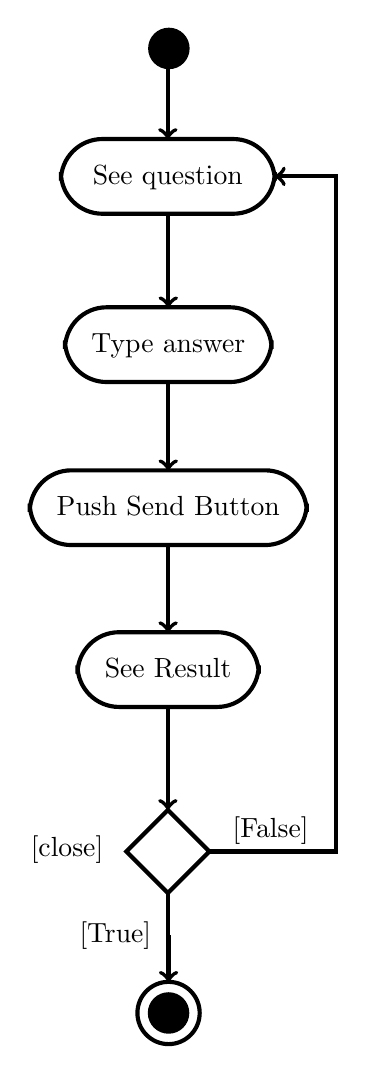
\begin{tikzpicture}[even odd rule]
\pgftransformxscale{1.000000}
\pgftransformyscale{-1.000000}
\definecolor{dialinecolor}{rgb}{0.000000, 0.000000, 0.000000}
\pgfsetstrokecolor{dialinecolor}
\pgfsetstrokeopacity{1.000000}
\definecolor{diafillcolor}{rgb}{1.000000, 1.000000, 1.000000}
\pgfsetfillcolor{diafillcolor}
\pgfsetfillopacity{1.000000}
\pgfsetlinewidth{0.100000\du}
\pgfsetdash{}{0pt}
\definecolor{diafillcolor}{rgb}{0.000000, 0.000000, 0.000000}
\pgfsetfillcolor{diafillcolor}
\pgfsetfillopacity{1.000000}
\pgfpathellipse{\pgfpoint{13.051186\du}{4.436548\du}}{\pgfpoint{0.500000\du}{0\du}}{\pgfpoint{0\du}{0.500000\du}}
\pgfusepath{fill}
\pgfsetlinewidth{0.100000\du}
\pgfsetdash{}{0pt}
\definecolor{diafillcolor}{rgb}{1.000000, 1.000000, 1.000000}
\pgfsetfillcolor{diafillcolor}
\pgfsetfillopacity{1.000000}
\pgfpathellipse{\pgfpoint{13.043589\du}{27.672360\du}}{\pgfpoint{0.750000\du}{0\du}}{\pgfpoint{0\du}{0.750000\du}}
\pgfusepath{fill}
\definecolor{dialinecolor}{rgb}{0.000000, 0.000000, 0.000000}
\pgfsetstrokecolor{dialinecolor}
\pgfsetstrokeopacity{1.000000}
\pgfpathellipse{\pgfpoint{13.043589\du}{27.672360\du}}{\pgfpoint{0.750000\du}{0\du}}{\pgfpoint{0\du}{0.750000\du}}
\pgfusepath{stroke}
\definecolor{diafillcolor}{rgb}{0.000000, 0.000000, 0.000000}
\pgfsetfillcolor{diafillcolor}
\pgfsetfillopacity{1.000000}
\pgfpathellipse{\pgfpoint{13.043589\du}{27.672360\du}}{\pgfpoint{0.500000\du}{0\du}}{\pgfpoint{0\du}{0.500000\du}}
\pgfusepath{fill}
\pgfsetlinewidth{0.100000\du}
\pgfsetdash{}{0pt}
{\pgfsetcornersarced{\pgfpoint{1.000000\du}{1.000000\du}}\definecolor{diafillcolor}{rgb}{1.000000, 1.000000, 1.000000}
\pgfsetfillcolor{diafillcolor}
\pgfsetfillopacity{1.000000}
\fill (10.450000\du,6.618969\du)--(10.450000\du,8.418969\du)--(15.602500\du,8.418969\du)--(15.602500\du,6.618969\du)--cycle;
}{\pgfsetcornersarced{\pgfpoint{1.000000\du}{1.000000\du}}\definecolor{dialinecolor}{rgb}{0.000000, 0.000000, 0.000000}
\pgfsetstrokecolor{dialinecolor}
\pgfsetstrokeopacity{1.000000}
\draw (10.450000\du,6.618969\du)--(10.450000\du,8.418969\du)--(15.602500\du,8.418969\du)--(15.602500\du,6.618969\du)--cycle;
}% setfont left to latex
\definecolor{dialinecolor}{rgb}{0.000000, 0.000000, 0.000000}
\pgfsetstrokecolor{dialinecolor}
\pgfsetstrokeopacity{1.000000}
\definecolor{diafillcolor}{rgb}{0.000000, 0.000000, 0.000000}
\pgfsetfillcolor{diafillcolor}
\pgfsetfillopacity{1.000000}
\node[anchor=base,inner sep=0pt, outer sep=0pt,color=dialinecolor] at (13.026250\du,7.713022\du){See question};
\pgfsetlinewidth{0.100000\du}
\pgfsetdash{}{0pt}
{\pgfsetcornersarced{\pgfpoint{1.000000\du}{1.000000\du}}\definecolor{diafillcolor}{rgb}{1.000000, 1.000000, 1.000000}
\pgfsetfillcolor{diafillcolor}
\pgfsetfillopacity{1.000000}
\fill (10.550000\du,10.672526\du)--(10.550000\du,12.472526\du)--(15.525618\du,12.472526\du)--(15.525618\du,10.672526\du)--cycle;
}{\pgfsetcornersarced{\pgfpoint{1.000000\du}{1.000000\du}}\definecolor{dialinecolor}{rgb}{0.000000, 0.000000, 0.000000}
\pgfsetstrokecolor{dialinecolor}
\pgfsetstrokeopacity{1.000000}
\draw (10.550000\du,10.672526\du)--(10.550000\du,12.472526\du)--(15.525618\du,12.472526\du)--(15.525618\du,10.672526\du)--cycle;
}% setfont left to latex
\definecolor{dialinecolor}{rgb}{0.000000, 0.000000, 0.000000}
\pgfsetstrokecolor{dialinecolor}
\pgfsetstrokeopacity{1.000000}
\definecolor{diafillcolor}{rgb}{0.000000, 0.000000, 0.000000}
\pgfsetfillcolor{diafillcolor}
\pgfsetfillopacity{1.000000}
\node[anchor=base,inner sep=0pt, outer sep=0pt,color=dialinecolor] at (13.037809\du,11.766579\du){Type answer};
\pgfsetlinewidth{0.100000\du}
\pgfsetdash{}{0pt}
{\pgfsetcornersarced{\pgfpoint{1.000000\du}{1.000000\du}}\definecolor{diafillcolor}{rgb}{1.000000, 1.000000, 1.000000}
\pgfsetfillcolor{diafillcolor}
\pgfsetfillopacity{1.000000}
\fill (9.700000\du,14.600000\du)--(9.700000\du,16.400000\du)--(16.372500\du,16.400000\du)--(16.372500\du,14.600000\du)--cycle;
}{\pgfsetcornersarced{\pgfpoint{1.000000\du}{1.000000\du}}\definecolor{dialinecolor}{rgb}{0.000000, 0.000000, 0.000000}
\pgfsetstrokecolor{dialinecolor}
\pgfsetstrokeopacity{1.000000}
\draw (9.700000\du,14.600000\du)--(9.700000\du,16.400000\du)--(16.372500\du,16.400000\du)--(16.372500\du,14.600000\du)--cycle;
}% setfont left to latex
\definecolor{dialinecolor}{rgb}{0.000000, 0.000000, 0.000000}
\pgfsetstrokecolor{dialinecolor}
\pgfsetstrokeopacity{1.000000}
\definecolor{diafillcolor}{rgb}{0.000000, 0.000000, 0.000000}
\pgfsetfillcolor{diafillcolor}
\pgfsetfillopacity{1.000000}
\node[anchor=base,inner sep=0pt, outer sep=0pt,color=dialinecolor] at (13.036250\du,15.694053\du){Push Send Button};
\pgfsetlinewidth{0.100000\du}
\pgfsetdash{}{0pt}
{\pgfsetcornersarced{\pgfpoint{1.000000\du}{1.000000\du}}\definecolor{diafillcolor}{rgb}{1.000000, 1.000000, 1.000000}
\pgfsetfillcolor{diafillcolor}
\pgfsetfillopacity{1.000000}
\fill (10.850000\du,18.500000\du)--(10.850000\du,20.300000\du)--(15.215000\du,20.300000\du)--(15.215000\du,18.500000\du)--cycle;
}{\pgfsetcornersarced{\pgfpoint{1.000000\du}{1.000000\du}}\definecolor{dialinecolor}{rgb}{0.000000, 0.000000, 0.000000}
\pgfsetstrokecolor{dialinecolor}
\pgfsetstrokeopacity{1.000000}
\draw (10.850000\du,18.500000\du)--(10.850000\du,20.300000\du)--(15.215000\du,20.300000\du)--(15.215000\du,18.500000\du)--cycle;
}% setfont left to latex
\definecolor{dialinecolor}{rgb}{0.000000, 0.000000, 0.000000}
\pgfsetstrokecolor{dialinecolor}
\pgfsetstrokeopacity{1.000000}
\definecolor{diafillcolor}{rgb}{0.000000, 0.000000, 0.000000}
\pgfsetfillcolor{diafillcolor}
\pgfsetfillopacity{1.000000}
\node[anchor=base,inner sep=0pt, outer sep=0pt,color=dialinecolor] at (13.032500\du,19.594053\du){See Result};
\pgfsetlinewidth{0.100000\du}
\pgfsetdash{}{0pt}
\definecolor{diafillcolor}{rgb}{1.000000, 1.000000, 1.000000}
\pgfsetfillcolor{diafillcolor}
\pgfsetfillopacity{1.000000}
\fill (12.027613\du,23.782071\du)--(13.027613\du,22.782071\du)--(14.027613\du,23.782071\du)--(13.027613\du,24.782071\du)--cycle;
\definecolor{dialinecolor}{rgb}{0.000000, 0.000000, 0.000000}
\pgfsetstrokecolor{dialinecolor}
\pgfsetstrokeopacity{1.000000}
\draw (12.027613\du,23.782071\du)--(13.027613\du,22.782071\du)--(14.027613\du,23.782071\du)--(13.027613\du,24.782071\du)--cycle;
% setfont left to latex
\definecolor{dialinecolor}{rgb}{0.000000, 0.000000, 0.000000}
\pgfsetstrokecolor{dialinecolor}
\pgfsetstrokeopacity{1.000000}
\definecolor{diafillcolor}{rgb}{0.000000, 0.000000, 0.000000}
\pgfsetfillcolor{diafillcolor}
\pgfsetfillopacity{1.000000}
\node[anchor=base west,inner sep=0pt,outer sep=0pt,color=dialinecolor] at (9.725388\du,23.910461\du){\ensuremath{[}close\ensuremath{]}};
% setfont left to latex
\definecolor{dialinecolor}{rgb}{0.000000, 0.000000, 0.000000}
\pgfsetstrokecolor{dialinecolor}
\pgfsetstrokeopacity{1.000000}
\definecolor{diafillcolor}{rgb}{0.000000, 0.000000, 0.000000}
\pgfsetfillcolor{diafillcolor}
\pgfsetfillopacity{1.000000}
\node[anchor=base west,inner sep=0pt,outer sep=0pt,color=dialinecolor] at (10.899436\du,25.968200\du){\ensuremath{[}True\ensuremath{]}};
% setfont left to latex
\definecolor{dialinecolor}{rgb}{0.000000, 0.000000, 0.000000}
\pgfsetstrokecolor{dialinecolor}
\pgfsetstrokeopacity{1.000000}
\definecolor{diafillcolor}{rgb}{0.000000, 0.000000, 0.000000}
\pgfsetfillcolor{diafillcolor}
\pgfsetfillopacity{1.000000}
\node[anchor=base west,inner sep=0pt,outer sep=0pt,color=dialinecolor] at (14.587006\du,23.456328\du){\ensuremath{[}False\ensuremath{]}};
\pgfsetlinewidth{0.100000\du}
\pgfsetbuttcap
\pgfsetdash{}{0pt}
{
\definecolor{diafillcolor}{rgb}{0.000000, 0.000000, 0.000000}
\pgfsetfillcolor{diafillcolor}
\pgfsetfillopacity{1.000000}
% was here!!!
\pgfsetarrowsend{to}
\definecolor{dialinecolor}{rgb}{0.000000, 0.000000, 0.000000}
\pgfsetstrokecolor{dialinecolor}
\pgfsetstrokeopacity{1.000000}
\draw (13.051186\du,4.936548\du)--(13.026250\du,4.936548\du)--(13.026250\du,6.618969\du);
}
% setfont left to latex
\pgfsetlinewidth{0.100000\du}
\pgfsetbuttcap
\pgfsetdash{}{0pt}
{
\definecolor{diafillcolor}{rgb}{0.000000, 0.000000, 0.000000}
\pgfsetfillcolor{diafillcolor}
\pgfsetfillopacity{1.000000}
% was here!!!
\pgfsetarrowsend{to}
\definecolor{dialinecolor}{rgb}{0.000000, 0.000000, 0.000000}
\pgfsetstrokecolor{dialinecolor}
\pgfsetstrokeopacity{1.000000}
\draw (14.027613\du,23.782071\du)--(17.079834\du,23.782071\du)--(17.079834\du,7.518969\du)--(15.602500\du,7.518969\du);
}
% setfont left to latex
\pgfsetlinewidth{0.100000\du}
\pgfsetbuttcap
\pgfsetdash{}{0pt}
{
\definecolor{diafillcolor}{rgb}{0.000000, 0.000000, 0.000000}
\pgfsetfillcolor{diafillcolor}
\pgfsetfillopacity{1.000000}
% was here!!!
\pgfsetarrowsend{to}
\definecolor{dialinecolor}{rgb}{0.000000, 0.000000, 0.000000}
\pgfsetstrokecolor{dialinecolor}
\pgfsetstrokeopacity{1.000000}
\draw (13.026250\du,8.418969\du)--(13.026250\du,9.545748\du)--(13.037809\du,9.545748\du)--(13.037809\du,10.672526\du);
}
% setfont left to latex
\pgfsetlinewidth{0.100000\du}
\pgfsetbuttcap
\pgfsetdash{}{0pt}
{
\definecolor{diafillcolor}{rgb}{0.000000, 0.000000, 0.000000}
\pgfsetfillcolor{diafillcolor}
\pgfsetfillopacity{1.000000}
% was here!!!
\pgfsetarrowsend{to}
\definecolor{dialinecolor}{rgb}{0.000000, 0.000000, 0.000000}
\pgfsetstrokecolor{dialinecolor}
\pgfsetstrokeopacity{1.000000}
\draw (13.037809\du,12.472526\du)--(13.037809\du,13.536263\du)--(13.036250\du,13.536263\du)--(13.036250\du,14.600000\du);
}
% setfont left to latex
\pgfsetlinewidth{0.100000\du}
\pgfsetbuttcap
\pgfsetdash{}{0pt}
{
\definecolor{diafillcolor}{rgb}{0.000000, 0.000000, 0.000000}
\pgfsetfillcolor{diafillcolor}
\pgfsetfillopacity{1.000000}
% was here!!!
\pgfsetarrowsend{to}
\definecolor{dialinecolor}{rgb}{0.000000, 0.000000, 0.000000}
\pgfsetstrokecolor{dialinecolor}
\pgfsetstrokeopacity{1.000000}
\draw (13.036250\du,16.400000\du)--(13.036250\du,17.450000\du)--(13.032500\du,17.450000\du)--(13.032500\du,18.500000\du);
}
% setfont left to latex
\pgfsetlinewidth{0.100000\du}
\pgfsetbuttcap
\pgfsetdash{}{0pt}
{
\definecolor{diafillcolor}{rgb}{0.000000, 0.000000, 0.000000}
\pgfsetfillcolor{diafillcolor}
\pgfsetfillopacity{1.000000}
% was here!!!
\pgfsetarrowsend{to}
\definecolor{dialinecolor}{rgb}{0.000000, 0.000000, 0.000000}
\pgfsetstrokecolor{dialinecolor}
\pgfsetstrokeopacity{1.000000}
\draw (13.032500\du,20.300000\du)--(13.032500\du,21.541035\du)--(13.027613\du,21.541035\du)--(13.027613\du,22.782071\du);
}
% setfont left to latex
\pgfsetlinewidth{0.100000\du}
\pgfsetbuttcap
\pgfsetdash{}{0pt}
{
\definecolor{diafillcolor}{rgb}{0.000000, 0.000000, 0.000000}
\pgfsetfillcolor{diafillcolor}
\pgfsetfillopacity{1.000000}
% was here!!!
\pgfsetarrowsend{to}
\definecolor{dialinecolor}{rgb}{0.000000, 0.000000, 0.000000}
\pgfsetstrokecolor{dialinecolor}
\pgfsetstrokeopacity{1.000000}
\draw (13.027613\du,24.782071\du)--(13.027613\du,25.852216\du)--(13.043589\du,25.852216\du)--(13.043589\du,26.922360\du);
}
% setfont left to latex
\end{tikzpicture}
